\section{Unterteilungen und Minoren}

\textbf{Definition}: Sei $G=(V,E)$ ein Graph, $e=uv$ eine Kante. Dann ist die \textbf{Unterteilung von $\boldsymbol{e}$ in $\boldsymbol{G}$} der Graph $G\circ e=(V',E')$ mit
\begin{itemize}
	\item $V'=V+\{w\}$
	\item $E'=(E\setminus \{uv\})+\{uw,vw\}$
\end{itemize}
\bigskip
\textbf{Beobachtung}: $G$ planar $\iff$ $G\circ e$ planar\\

\textbf{Definition}: Graph $G$ ist eine \textbf{Unterteilung von $\boldsymbol{H}$} wenn $G=((H \circ e_1)\circ e_2)\cdots)\circ e_k$.
Wir sagen auch $G$ ist $\boldsymbol{H}$\textbf{-Unterteilung}.
Graph $G$ \textbf{enthält eine $\boldsymbol{H}$-Unterteilung}, wenn ein Teilgraph $G'\subseteq G$ eine $H$-Unterteilung ist.

\begin{center}
	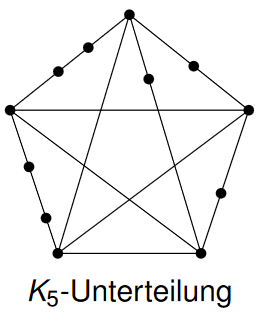
\includegraphics[width=0.17\textwidth]{images/k5-unterteilung.png}
\end{center}

\textbf{Beobachtung}: 
\begin{itemize}
	\item $K_5$- und $K_{3,3}$-Unterteilungen sind nicht-planar
	\item Jeder Graph der eine $K_5$ oder $K_{3,3}$-Unterteilung enthält, ist nicht planar
\end{itemize}
\bigskip
\textbf{Satz von Kuratowski}: $G$ ist planar $\iff$ $G$ enthält keine $K_5$- oder $K_{3,3}$-Unterteilung

\textit{Beweis}: \enquote{$\Rightarrow$} folgt aus obiger Beobachtung. Die Rückrichtung ist komplizierter und beweisen wir später.\\

\textbf{Definition}: Sei $G=(V,E)$ ein Graph, $e=uv$ eine Kante. Der Graph $G/e=(V',E')$ ist der Graph, der durch Kontrahieren der Kante $\boldsymbol{e}$ entsteht, genauer:
\begin{itemize}
	\item $V'=V\setminus\{u,v\}+\{w\}$
	\item $E'=E(G-u-v)\cup\{wa\mid au\in E \text{ oder } av\in E\}$
\end{itemize}
Diesen Prozess nennt man auch \textbf{Kantenkontraktion}. Dabei können Multikanten und Schlaufen entstehen.
\begin{center}
	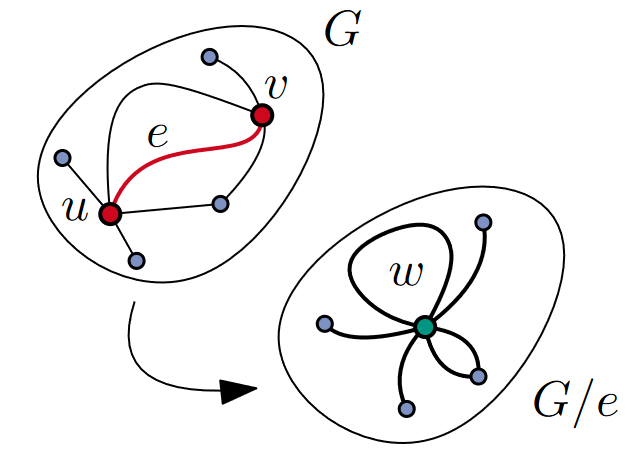
\includegraphics[width=0.3\textwidth]{images/kantenkontraktion.png}
\end{center}
\bigskip
\textbf{Definition}: Graph $H$ ist \textbf{Minor von} $\boldsymbol{G}$, wenn $H$ aus $G$ durch eine Folge von Kantenkontraktionen entsteht, also $H=((G/e_1)/e_2\cdots)/e_k$. Wir sagen dann auch: $G$ ist ein \textbf{$\boldsymbol{H}$-Minor} ($H$ ist der kleinere Graph, $G$ der Größere).\\

\textbf{Beobachtung}:
\begin{itemize}
	\item $G$ planar $\implies$ $G/e$ planar
	\item $G$ enthält $K_5$- oder $K_{3,3}$-Minor $\implies$ $G$ nicht planar
\end{itemize}
\bigskip
\textbf{Satz von Wagner}: $G$ planar $\iff$ $G$ enthält keinen $K_5$- oder $K_{3,3}$-Minor\\

\textbf{Lemma}: $G$ enthält $H$-Unterteilung $\implies $ $G$ enthält $H$-Minor

\textit{Beweis}: Kontrahiere durch Unterteilung entstandene Knoten zu ursprünglich adjazenten Knoten.
\begin{center}
	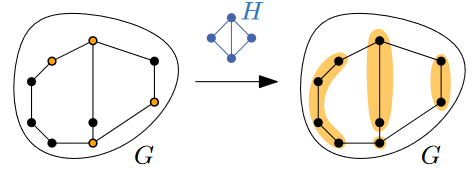
\includegraphics[width=0.35\textwidth]{images/um-skizze.png}
\end{center}
\pagebreak

\textbf{Es sind also äquivalent}:
\begin{enumerate}
	\item $G$ ist nicht planar
	\item $G$ enthält $K_5$- oder $K_{3,3}$-Minor
	\item $G$ enthält $K_5$- oder $K_{3,3}$-Unterteilung
\end{enumerate}

$(3)\implies(2)\implies(1)$ wurde schon bewiesen, $(1)\implies(2)\implies(3)$ müssen wir noch beweisen. Wir beginnen mit $(1)\implies(2)$.\\

\textit{Beweis von Wagner}: Es muss nur noch die Rückrichtung beweisen werden. Sei hierfür $G$ ein nicht-planarer Graph. Wir müssen einen $K_5$- oder $K_{3,3}$-Minor in $G$ finden. O.B.d.A. sei $G$ sogar minimal nicht-planar, d.h.
\begin{itemize}
	\item $G-v$ ist planar für jeden Knoten $v\in V$
	\item $G-e$ ist planar für jede Kante $e\in E$
	\item $G/e$ ist planar für jede Kante $e\in E$
\end{itemize}

Beweise zunächst folgendes Lemma:\\

\textbf{Lemma}: Sei $G$ minimal nicht-planar, $xy\in E(G)$. Dann ist $G-x-y$ ein Kreis.